% !TEX TS-program = XeLaTeX
% !TEX spellcheck = en-US
\documentclass[aspectratio=169]{beamer}

% Choose your theme
\usetheme{example}

\title{Lecture 4:\\ Classification Analysis}
\institute{GRA4160: Predictive Modelling with Machine Learning}
\date{January 30, 2025} 
\author{Vegard H\o ghaug Larsen}

%------------------------------------------------------------------------------
\begin{document}
%------------------------------------------------------------------------------
\maketitle

\frame{
    \frametitle{Plan for Today}
    \begin{itemize}
        \item \textbf{Recap} from last week: LDA and Regularized Regression
        \item \textbf{Logistic Regression}
        \item \textbf{Decision Trees}
        \item \textbf{Exercise: Recognizing handwritten digits}
    \end{itemize}
}

% ------------------------------------------------------------
%   LDA Recap
% ------------------------------------------------------------
\begin{frame}
    \frametitle{Recap: Linear Discriminant Analysis (LDA)}
    \begin{itemize}
        \item \textbf{Purpose:}
            \begin{itemize}
                \item Supervised classification \& dimensionality reduction.
                \item Projects data onto a lower-dimensional space to maximize class separation.
            \end{itemize}
        \item \textbf{When to Use:}
            \begin{itemize}
                \item Two or more well-separated classes with similar covariance matrices.
                \item Need for interpretable linear boundaries and reduced dimensionality.
            \end{itemize}
        \item \textbf{Mathematical Core:}
            \begin{itemize}
                \item Defines scatter matrices: \(\mathbf{S}_B\) (between-class) and \(\mathbf{S}_W\) (within-class).
                \item Objective: 
                \[
                    \max_{\mathbf{w}} \; \frac{\mathbf{w}^T \mathbf{S}_B \mathbf{w}}{\mathbf{w}^T \mathbf{S}_W \mathbf{w}}.
                \]
            \end{itemize}
    \end{itemize}
\end{frame}

\begin{frame}
    \frametitle{Recap: LDA Assumptions \& Practical Tips}
    \begin{itemize}
        \item \textbf{Key Assumptions:}
            \begin{enumerate}
                \item Each class follows (approximately) a normal (Gaussian) distribution.
                \item All classes share the same covariance matrix.
                \item Features are ideally uncorrelated, but mild correlations are often acceptable.
            \end{enumerate}
        \item \textbf{Implications:}
            \begin{itemize}
                \item If covariances differ significantly, consider Quadratic Discriminant Analysis (QDA).
                \item LDA can be robust to mild violations of normality.
            \end{itemize}
        \item \textbf{Practical Tips:}
            \begin{itemize}
                \item Scale/standardize data to stabilize covariance estimation.
                \item Use cross-validation to evaluate classification performance (e.g., confusion matrices).
                \item Works well with moderate-to-large datasets that have reasonable class separation.
            \end{itemize}
        \item \textbf{Takeaway:} 
            A simple, interpretable linear boundary with dimensionality reduction under Gaussian assumptions.
    \end{itemize}
\end{frame}

% ------------------------------------------------------------
%   Regularized Regression Recap
% ------------------------------------------------------------
\begin{frame}
    \frametitle{Recap: Regularized Regression (Ridge, Lasso, Elastic Net)}
    \begin{itemize}
        \item \textbf{Motivation:} Mitigate overfitting by penalizing large coefficients.
        \item \textbf{Methods Overview:}
            \begin{itemize}
                \item \textbf{Ridge (L2):}
                    \begin{itemize}
                        \item Shrinks coefficients (rarely to exactly zero).
                        \item Useful for handling multicollinearity.
                    \end{itemize}
                \item \textbf{Lasso (L1):}
                    \begin{itemize}
                        \item Can set some coefficients to zero (\emph{feature selection}).
                        \item Often helpful in high-dimensional settings.
                    \end{itemize}
                \item \textbf{Elastic Net (L1 + L2):}
                    \begin{itemize}
                        \item Balances the strengths of Ridge and Lasso.
                        \item Two hyperparameters: overall strength (\(\lambda\)) + mixing ratio (\(\alpha\)).
                    \end{itemize}
            \end{itemize}
        \item \textbf{Choosing \(\lambda\):}
            \begin{itemize}
                \item Use cross-validation to find the best bias-variance trade-off.
                \item Standardize features before applying the penalty terms.
            \end{itemize}
        \item \textbf{Key Takeaway:}
            Regularization improves generalization, reduces overfitting, and can do feature selection (Lasso/Elastic Net).
    \end{itemize}
\end{frame}

% ------------------------------------------------------------
%   Logistic Regression
% ------------------------------------------------------------
\frame{
    \frametitle{Logistic Regression}
    \begin{itemize}
        \item A \textbf{binary classification} model (e.g., yes/no, success/failure).
        \pause
        \item Assumes a linear relationship between predictors \(\mathbf{x}\) and the \emph{log-odds} of the outcome:
        \[
            \log\!\Bigl(\tfrac{p}{1-p}\Bigr) = \beta_0 + \beta_1x_1 + \cdots + \beta_k x_k
        \]
        \pause
        \item The log-odds transformation (logit) ensures predicted probabilities are always in \([0,1]\).
        \pause
        \item Often fit by \emph{maximum likelihood} (minimizing negative log-likelihood).
        \pause
        \item Can be extended to multi-class problems (via One-vs-All or Multinomial/Softmax).
    \end{itemize}
}

% ------------------------------------------------------------
%   Logistic Function
% ------------------------------------------------------------
\frame{
    \frametitle{The Logistic (Sigmoid) Function}
    \begin{minipage}{0.55\textwidth}
        \begin{itemize}
            \item Maps \(\mathbb{R}\) to \([0,1]\), producing valid probabilities.
            \[
                f(z) = \frac{1}{1 + e^{-z}}
            \]
            \item As \(z \rightarrow \infty\), \(f(z) \rightarrow 1\); as \(z \rightarrow -\infty\), \(f(z) \rightarrow 0\).
        \end{itemize}
    \end{minipage}
    \hfill
    \begin{minipage}{0.4\textwidth}
        \centering
        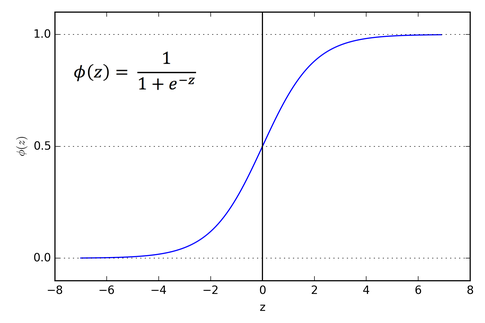
\includegraphics[width=\linewidth]{../figures/sigmoid.png} % Replace with actual filename
    \end{minipage}
    \pause
    Relates directly to the log-odds:
    \[
        p = \frac{1}{1 + e^{-z}} = \frac{e^z}{1 + e^z}
    \]
}


\frame{
    \frametitle{Relation: Log-odds, Probability, and Sigmoid}
    \[
        \log\!\Bigl(\tfrac{p}{1-p}\Bigr) = z = \beta_0 + \beta_1x_1 + \cdots + \beta_kx_k
    \]
    \pause
    \[
        \tfrac{p}{1-p} = e^z \quad \Rightarrow \quad p = \frac{e^z}{1 + e^z}
    \]
    \pause
    \[
        p = \frac{1}{1 + e^{-z}} \quad \text{(the sigmoid)}
    \]
    \begin{itemize}
        \item Changing \(z\) by 1 unit multiplies the odds \(\frac{p}{1-p}\) by \(e^1 \approx 2.718.\)
    \end{itemize}
}

% ------------------------------------------------------------
%   Decision Trees
% ------------------------------------------------------------
\frame{
    \frametitle{Decision Trees}
    \begin{itemize}
        \item A \textbf{non-parametric} method for classification and regression.
        \pause
        \item The data is repeatedly \emph{split} into subsets based on feature thresholds, growing a tree structure.
        \pause
        \item Each \textbf{split} is chosen to maximize the purity of the resulting subsets (minimize impurity).
        \pause
        \item \textbf{Advantages}: Interpretability, handles mixed feature types, no need for feature scaling.
        \item \textbf{Drawbacks}: Can overfit if not pruned, can be unstable (high variance) for small data.
    \end{itemize}
}

\frame{
    \frametitle{Training a Decision Tree}
    \begin{itemize}
        \item Constructed \emph{recursively}:
        \begin{itemize}
            \item Choose a feature + threshold to best split the data (based on impurity).
            \item Split the data into two (or more) subsets.
            \item Repeat the process on each subset until a stopping criterion is met.
        \end{itemize}
        \pause
        \item Stopping criteria:
        \begin{itemize}
            \item Maximum depth reached.
            \item Fewer samples in a node than the minimum required for a split.
            \item Impurity improvement is below a certain threshold.
        \end{itemize}
    \end{itemize}
}

\frame{
    \frametitle{Impurity Measures: Gini vs. Entropy}
    \begin{itemize}
        \item \textbf{Gini Index} (\(G\)):
            \[
                G = \sum_{i=1}^{C} p_i (1 - p_i) = 1 - \sum_{i=1}^{C} p_i^2
            \]
            \item Measures the chance of misclassification if you pick a label at random.
            \item \(G = 0\) means perfectly pure (all samples in one class).
        \pause
        \item \textbf{Entropy} (\(\mathcal{H}\)):
            \[
                \mathcal{H} = -\sum_{i=1}^{C} p_i \log_2(p_i)
            \]
            \item Based on the concept of information theory (uncertainty).
            \item \(\mathcal{H} = 0\) means a perfectly pure subset.
        \pause
        \item \textbf{Information Gain}: The reduction in impurity from a split.
    \end{itemize}
}

\end{document}
